\documentclass{article}

% Language setting
% Replace `english' with e.g. `spanish' to change the document language
\usepackage[italian]{babel}

% Set page size and margins
\usepackage[a4paper,top=3cm,bottom=3cm,left=3cm,right=3cm,marginparwidth=1.75cm]{geometry}

% Useful packages
% \usepackage{showframe}
% \usepackage{layout}
%comando per più righe su una cella di tabella
\newcommand{\quantities}[1]{%
  \begin{tabular}{@{}c@{}}\strut#1\strut\end{tabular}%
}
\usepackage[table]{xcolor}
\usepackage[dvipsnames, table]{xcolor}
\definecolor{light_orange}{HTML}{FFB88E}
\usepackage{amsmath}
\usepackage{graphicx}
\usepackage[colorlinks=true, allcolors=blue]{hyperref}
\usepackage{tikz}
\usetikzlibrary{shapes, backgrounds, mindmap, trees}
\usepackage{fancyhdr}
\usetikzlibrary{positioning}
\usepackage[inkscapeformat=png]{svg}
\usepackage{caption}

\usepackage{hyperref}
\usepackage{lastpage}
\usepackage{moresize}
\usepackage{paracol}
\usepackage{enumitem}
\usepackage{nicematrix}
\usepackage{tabularx}
\usepackage{parskip}
\usepackage{fontspec}
\usepackage{style}
\usepackage{float}
\hypersetup{
    colorlinks=true, % Imposta i collegamenti come testo colorato anziché riquadri intorno al testo
    linkcolor=black,  % Colore dei link alle sezioni
    filecolor=black, % Colore dei link ai file
    urlcolor=black, % Colore dei link agli URL
}

\setmainfont{Poppins}[
    Path=./Poppins/,
    Extension = .ttf,
    UprightFont=*-Regular,
    BoldFont=*-Bold,
    ItalicFont=*-Italic,
    BoldItalicFont=*-BoldItalic
    ]

\title{Titolo}
\author{SWEetCode}

\begin{document}
% \layout

\begin{titlepage}
    \thispagestyle{empty}
    \begin{tikzpicture}[remember picture, overlay]
        % TRIANGOLI
        \draw[fill=secondarycolor, secondarycolor] (current page.north west) -- (current page.south west) -- (8.8, -28);
        \draw[fill=primarycolor, primarycolor] (-3, 5) -- (4, -13.6) -- (11, 5);

        % LOGO
        \node [xshift=-5cm, yshift=25cm] (logo) at (current page.south east) {\includesvg[width=6.5cm]{logo.svg}};

        % SWEETCODE - DATE
        \node [anchor=north east, align=right, xshift=-1.2cm, yshift=19.5cm, text=black] (sweetcode) at (current page.south east) {\fontsize{32pt}{36pt}\selectfont SWEetCode};
        \draw[line width=4pt, lightcol] ([xshift=-3cm, yshift=-0.37cm]sweetcode.south west) -- ([yshift=-0.37cm]sweetcode.south east);
        \node [anchor=north east, align=right, xshift=-1.2cm, yshift=17.7cm, text=black] (date) at (current page.south east){\fontsize{24pt}{24pt} \selectfont 2023-11-08 };

        % NOME FILE
        \node [anchor=north east, text width=15cm, align=right, xshift=-1.2cm, yshift=15cm, text=black] (titolo) at (current page.south east){\fontsize{40pt}{40pt}\textbf{Preventivo $  $ costi\\e $  $ impegni $  $ orari\\}}; % andare a capo con \\ 

        % BOX DATI PARTECIPANTI
        \node[anchor=north east, xshift=-1.2cm, yshift=12cm, minimum width=8cm] (box) at (current page.south east){};

        % VERSIONE
        \node[anchor=north west, align=left] (dati1) at (box.north west) {\fontsize{16pt}{16pt}\selectfont \textbf{}};
        % \draw[line width=4pt, lightcol] (dati1.south west) -- ([xshift=8cm]dati1.south west);
        \node[anchor=north west, align=left] (dati11) at (dati1.south west)
        {\fontsize{14pt}{14pt}\selectfont};

        % COMPONENTI DEL GRUPPO
        \node[anchor=north west, yshift=-1cm, align=left] (dati2) at (dati11.north west) {\fontsize{16pt}{16pt}\selectfont \textbf{Componenti del gruppo}};
        \draw[line width=4pt, lightcol] (dati2.south west) -- ([xshift=8cm]dati2.south west);
        \node[anchor=north west, align=left] (dati21) at (dati2.south west)
        {\fontsize{14pt}{14pt}\selectfont Bresolin G.};
        \node[anchor=north west, yshift=-0.7cm, align=left] (dati22) at (dati2.south west)
        {\fontsize{14pt}{14pt}\selectfont Campese M.};
        \node[anchor=north west, yshift=-1.4cm, align=left] (dati23) at (dati2.south west)
        {\fontsize{14pt}{14pt}\selectfont Ciriolo I.};
        \node[anchor=north west, yshift=-2.1cm, align=left] (dati24) at (dati2.south west)
        {\fontsize{14pt}{14pt}\selectfont Dugo A.};
        \node[anchor=north west, yshift=-2.8cm, align=left] (dati25) at (dati2.south west)
        {\fontsize{14pt}{14pt}\selectfont Feltrin E.};
        \node[anchor=north west, yshift=-3.5cm, align=left] (dati26) at (dati2.south west)
        {\fontsize{14pt}{14pt}\selectfont Michelon R.};
        \node[anchor=north west, yshift=-4.2cm, align=left] (dati27) at (dati2.south west)
        {\fontsize{14pt}{14pt}\selectfont Orlandi G.};
        
        % UNIPD - SWE
        \node [xshift=4.4cm, yshift=2.3cm, draw, secondarycolor, text=white] (uni) at (current page.south west) {\fontsize{20pt}{20pt} \selectfont Università di Padova};
        \node [xshift=0.65cm, yshift=0.7cm, draw, secondarycolor, text=white, below=of uni] (corso) {\fontsize{20pt}{20pt}\selectfont Ingegneria del Software};

        % FIRMA
        % \draw[line width=4pt, lightcol] ([xshift=-1.2cm, yshift=1.8cm]current page.south east) -- ([xshift=-8cm, yshift=1.8cm]current page.south east);
        % \node[anchor=north west, xshift=12.9cm, yshift=1.45cm, align=left] at (current page.south west)
        % {\fontsize{13pt}{13pt}\selectfont L'Amministratore: Feltrin E.};
        
    \end{tikzpicture}
\end{titlepage}

%Registro in ordine dalla più recente alla meno recente!
{\renewcommand{\arraystretch}{1.5}
\section*{Registro delle versioni}
\begin{tabularx}{\textwidth}{c|c|c|c|X}
\textbf{Versione} & \textbf{Data} & \quantities{\textbf{Responsabile di}\\\textbf{stesura}}& \textbf{Revisore} & \quantities{\textbf{Dettaglio e}\\\textbf{motivazioni}} \\
\hline
v0.0.1(23) & $2023-11-13$ & Campese M. & Feltrin E. & Modifiche correttive di versione e registro delle modifiche. \\
\hline
v0.0.1(17) & $2023-10-29$ & Dugo A.& Michelon R. & Preventivo, impegno orario suddivisioni e timeline.\\
\hline
v0.0.1(14) & $2023-10-28$ & Bresolin G. & Michelon R. & Sezione dei rischi e loro mitigazione.\\
\hline
v0.0.1(9) & $2023-10-27$ & Ciriolo I. & Michelon R. &  Sezione dei ruoli e motivazioni.\\

\end{tabularx}}
\newpage

%INDICE
\tableofcontents
\newpage

\section{Suddivisione Ruoli}
La suddivisione delle ore per ruolo è stata eseguita tenendo conto del fatto che ogni componente del gruppo deve:
\begin{itemize}
    \item Ruotare su tutti i ruoli;
    \item Assumere ogni ruolo per un tempo totale congruo;
    \item Assumere non più di un ruolo alla volta.
\end{itemize}

%ANALISI RUOLI
\section{Analisi dei ruoli}
Si analizzano in questo paragrafo le motivazioni che hanno spinto il team a comporre la suddivisione delle ore assegnate ad ogni ruolo proposta in \textit{Impegno orario}. Si tiene successivamente conto del fatto che le ore di lavoro assegnate ad ogni membro del gruppo per ciascun ruolo sono state suddivise in modo leggermente diverso in base alle preferenze di ciascun componente.
\subsection{Analista}
Il ruolo dell'analista richiede meno ore rispetto alla media in quanto la figura si ritiene necessaria solo in determinate fasi dello sviluppo del progetto. Questo ruolo risulta infatti fondamentale nelle prime fasi (in particolar modo nell'analisi dei requisiti) e non segue lo svolgimento del lavoro fino al suo termine. 

\subsection{Progettista}
Il ruolo del progettista occupa un numero di ore medio-alto poichè considerato fondamentale. Il progettista aiuta a stabilire una struttura coerente per il progetto 
ed identifica le risorse necessarie per lo sviluppo. 
La figura svolge un ruolo cruciale nel garantire che il progetto sia ben strutturato, affidabile, efficiente, sicuro e in grado di soddisfare i requisiti specifici degli utenti finali.

\subsection{Programmatore}
Il programmatore è la figura a cui vengono assegnate più ore per ruolo in assoluto. Questo perchè ricopre un ruolo chiave all'interno dello sviluppo; il programmatore si occupa della traduzione delle specifiche e dei i requisiti del progetto in codice sorgente eseguibile e dell'ottimizzazione del codice per migliorare le prestazioni del progetto. Inoltre è responsabile dell'implementazione delle funzionalità avanzate all'interno del software (ciò richiede una comprensione approfondita dei linguaggi di programmazione e delle tecnologie pertinenti).

\subsection{Verificatore}
Il verificatore riveste un ruolo primario all'interno dello sviluppo del progetto, difatti gli vengono assegnate più ore di lavoro rispetto alla media. La figura deve garantire affidabilità e robustezza nei test e deve occuparsi del controllo di qualità del software e della documentazione in base agli standard imposto dal committente e dal team stesso (deve infatti avere una conoscenza approfondita del Way of working).

\subsection{Responsabile}
La figura del responsabile occupa un numero di ore leggermente inferiore alla media poichè costituisce il ruolo più economicamente dispendioso. Per questo motivo il team prevede di svolgere tale ruolo nel modo più efficiente possibile, riducendo (non al minimo indispensabile ma solo leggermente) la media delle ore per ruolo in modo da avere una resa massima per un costo medio-basso. Il responsabile garantisce il completamento del progetto  in modo tempestivo, efficiente e in linea con gli obiettivi e le aspettative del committente e verifica che la rotazione dei ruoli avvenga in modo corretto. Il ruolo richiede competenze nella gestione delle risorse e delle eventuali problematiche, nella comunicazione, e la capacità di pianificazione è fondamentale per il successo globale del progetto. 

\subsection{Amministratore di sistema}
Il ruolo dell'amministratore occupa il minor numero di ore (con l'analista) poichè si valuta che non richieda un elevato dispendio temporale. Complessivamente, la figura garantisce che l'ambiente e l'infrastruttura necessari per lo sviluppo e l'esecuzione del progetto siano robusti, sicuri ed affidabili. Il suo lavoro contribuisce alla stabilità complessiva del progetto.

\section{Preventivo costi}
Dopo una fase di analisi risultante nelle tabelle riportate sopra e considerate le precedenti osservazioni, il costo finale del progetto ammonta a \textbf{12845.00 €}.
\section{Impegno orario}

Ciascuno degli studenti del gruppo SWEetCode dedicherà un totale di 94 ore di lavoro produttivo durante lo svolgimento del Progetto.

{\renewcommand{\arraystretch}{1.2}
\begin{center}

    \begin{tabular}{l|c|c|c|c}
     \textbf{Ruoli} & \textbf{Costo Orario} & \textbf{Ore per Ruolo} & \quantities{\textbf{Ore Medie per}\\\textbf{Membro}} & \textbf{Percentuale Ore} \\
    \hline Responsabile & 30 & 70 & 10 & 10.6 \\
    \hline Amministratore & 20 & 63 & 9 & 9.6 \\
    \hline Verificatore & 15 & 168 & 24 & 25.5 \\
    \hline Progettista & 25 & 98 & 14 & 14.9 \\
    \hline Programmatore & 15 & 196 & 28 & 29.8 \\
    \hline Analista & 25 & 63 & 9 & 9.6\\
    \hline  & \textbf{Totale Costo} & \textbf{Totale Ore} & \quantities{\textbf{Totale Ore per}\\\textbf{Membro}}\\
    \hline  & \cellcolor{light_orange} 12845 & 658 & 94 \\
    \end{tabular}
\end{center}
\newpage
{\renewcommand{\arraystretch}{1.5}
\section{Suddivisione ore}
Nella tabella sottostante troviamo per ogni membro del gruppo l'ammontare delle ore rispetto al ruolo assunto.\\

\begin{center}
    \begin{tabular}{c|c|c|c|c|c|c|c}
        \textbf{Membri} & $\operatorname{\textbf{Re}}$ & $\mathrm{\textbf{Am}}$ & \textbf{An} & \textbf{Proj} & \textbf{Prgm} & \textbf{Ver} & \textbf{Tot} \\
        \hline Bresolin G. & 9 & 9 & 8 & 13 & 31 & 24 & 94 \\
        \hline Ciriolo I. & 11 & 11 & 10 & 16 & 27 & 19 & 94 \\
        \hline Campese M. & 10 & 10 & 8 & 15 & 26 & 25 & 94 \\
        \hline Dugo A. & 11 & 8 & 8 & 15 & 28 & 24 & 94 \\
        \hline Feltrin E. & 11 & 9 & 10 & 12 & 28 & 24 & 94 \\
        \hline Michelon R. & 9 & 8 & 10 & 13 & 30 & 24 & 94 \\
        \hline Orlandi G. & 9 & 8 & 9 & 14 & 26 & 28 & 94 
    \end{tabular}
\end{center}
\vspace{3em}
\subsection{Schema a torta di distribuzione ore ruoli}
    \begin{figure}[!h]
        \centering
        \includesvg{chart}
        %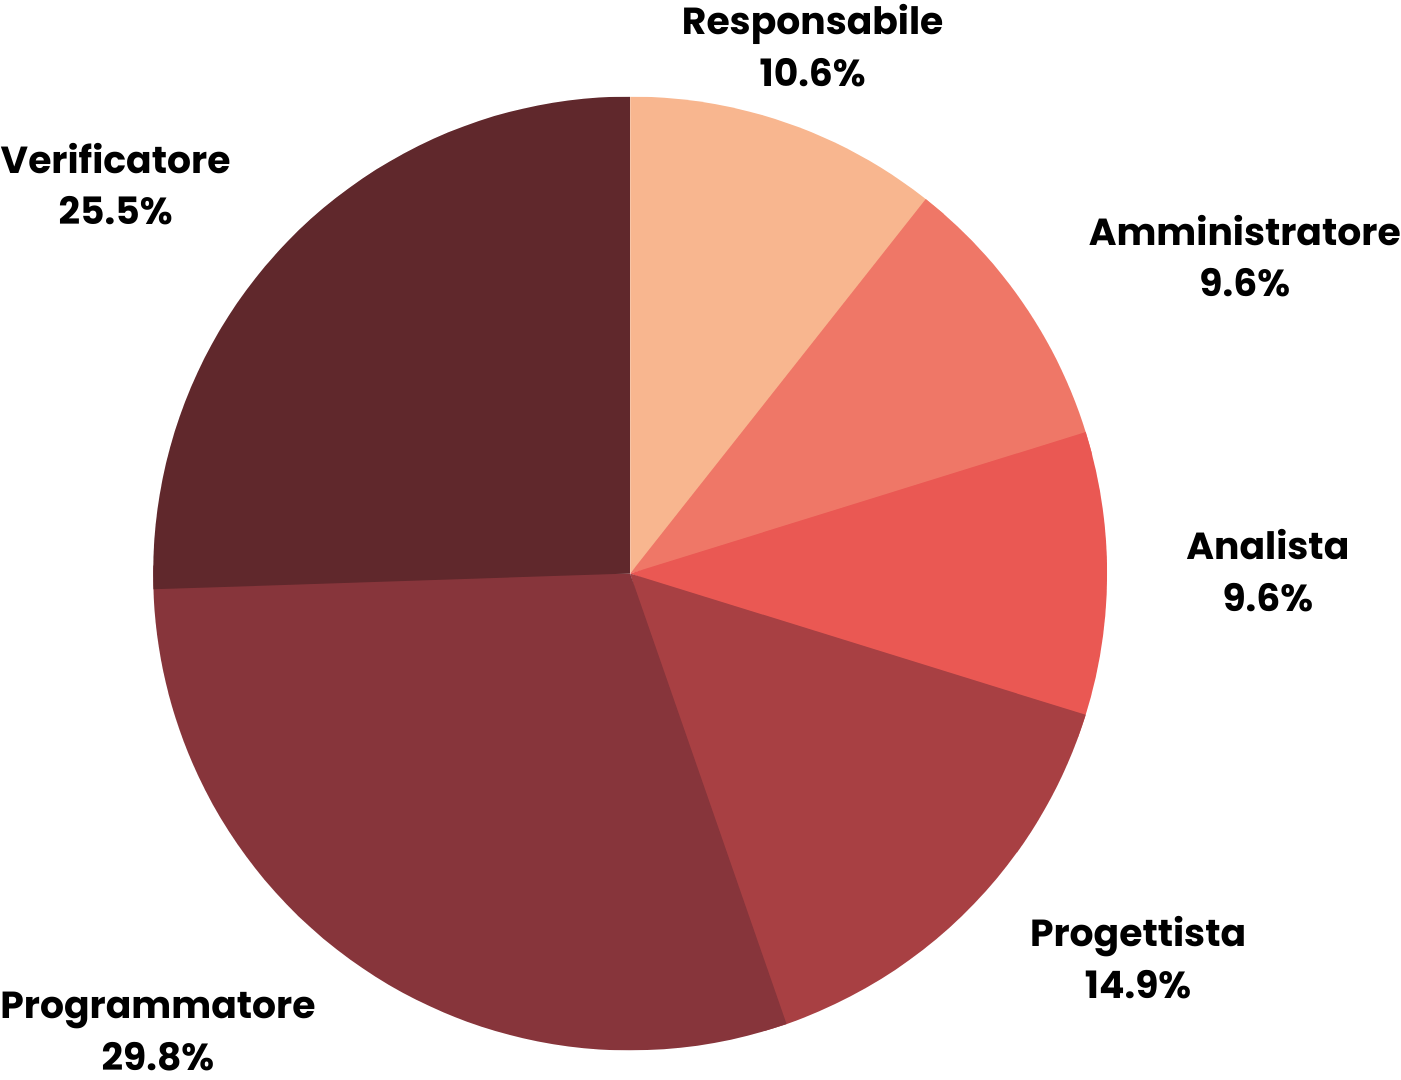
\includegraphics[width=10cm]{torta.png}
    \end{figure}

\newpage
\section{Scadenza di consegna}
Il gruppo stima di consegnare il prodotto finito relativo al capitolato C1, “Knowledge Management AI”, proposto dalla azienda AzzurroDigitale, entro : 8/04/2024.

    \subsection{Timeline periodi di consegna}
    \begin{figure}[!h]
        \centering
        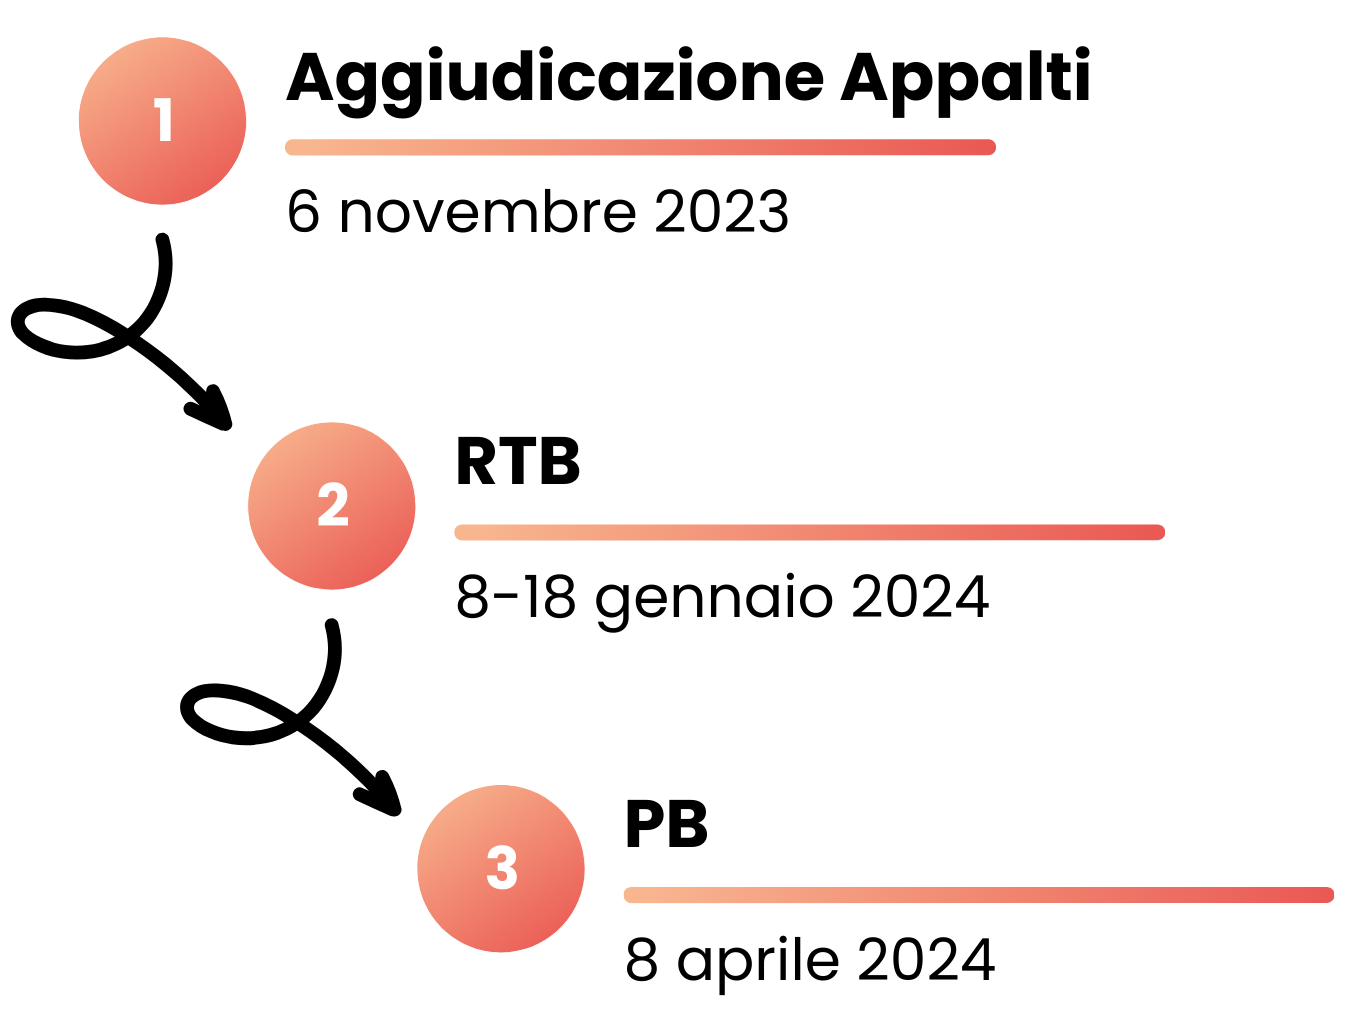
\includegraphics[width=10cm]{timeline.png}
    \end{figure}

    \subsection{Periodi di rallentamento}
    I possibili periodi di rallentamento che SWEetCode ha individuato sono tre: periodo Natalizio, sessione invernale e periodo Pasquale.
    In particolare i periodi si espandono nel seguente modo:\\
    \begin{center}
    \begin{tabular}{l|c|c}
         \textbf{Periodo} &  \textbf{Da} & \textbf{A} \\
            \hline Natalizio &  2023-12-23 & 2024-01-7 \\
            \hline Sessione invernale &  2024-01-22 & 2024-02-24 \\
            \hline Pasquale &  2023-03-29 & 2024-04-01 \\
    \end{tabular}
        \end{center}

    
    \subsection{Rischi e la loro mitigazione}
    In questa sezione vengono espresse le correlazioni tra il conteggio delle ore e i possibili rischi in cui il team potrebbe incombere, associati alle relative azioni di mitigazione che il gruppo si impegna a rispettare per ridurre gli impatti negativi.
            \subsubsection{Impegni personali}\\
            Il conteggio delle ore stabilito dal team tiene in considerazione uno scarto per eventuali imprevisti.\\
            Nella casistica in cui un membro del team non riesca ad eseguire i task a lui assegnati in un determinato lasso di tempo a causa di impegni personali esterni, il gruppo fa fronte a tale rischio coprendo l'intervallo non produttivo del componente con una suddivisione omogenea tra i restanti colleghi delle attività rimaste in sospeso. D'altra parte, il componente in causa si assume la responsabilità di dover recuperare le ore dedicate dal team per far fronte alla sua assenza totale o parziale;
            \subsubsection{Distribuzione non omogenea delle competenze}\\
            La distribuzione non omogenea delle competenze all'interno del gruppo potrebbe causare in determinate attività una discrepanza tra le stime di ore assegnate per il loro completamento e la loro effettiva realizzazione.\\
            Per mitigare tale rischio i membri del team si rendono disponibili ad una collaborazione interna, entro la quale chi predilige una certa competenza in determinate attività offre disponibilità a coloro che detengono abilità limitate.
            Attraverso questa assunzione di responsabilità, il team sostiene di poter portare a termine il progetto con il contributo collettivo di tutti i membri del gruppo;
            \subsubsection{Possibile difficoltà nella realizzazione di qualche attività}\\
            Durante lo sviluppo del progetto il gruppo potrebbe trovarsi a far fronte all'incombere di difficoltà nella realizzazione di qualche attività: i componenti interessati dovranno far presenti tali problematiche al resto del team e, in caso di disponibilità, i colleghi che detengono tempo da rendere a disposizione saranno incaricati di fornire assistenza.\\
            In ogni caso (ovvero sia nel caso in cui l'attività venga portata o termine o meno) tale difficoltà dovrà emergere nella riunione successiva più imminente, in modo da permettere una sua suddivisione in sotto-task più semplici: la suddivisione di un'attività complessa in attività più semplici è finalizzata all'ottimizzazione dell'efficienza operativa e alla riduzione dei tempi di completamento complessivi;
            \subsubsection{Sottostima del tempo necessario per soddisfare i requisiti}\\
            Nel caso in cui il team vada in contro ad una sottostima del tempo necessario per il completamento di un requisito tale errore di valutazione deve essere reso noto al team nel modo più rapido possibile, utilizzando i canali di comunicazione appropriati.\\
            Anche in questo caso i colleghi che detengono del tempo da rendere a disposizione saranno incaricati di fornire assistenza al fine di accorciare la distanza dal completamento del requisito.\\
            Nel caso di una sottostima, il team prima di procedere avvio di nuovi task si prende in carico una fase di riallineamento: in quanto questa fase dovrà durare il minor tempo possibile, tutte le risorse del gruppo saranno allocate per  assicurare il suo soddisfacimento, a meno di quelle necessarie per il proseguimento delle attività ad alta priorità e importanza che non possono essere interrotte.

\end{document}